% This file was created by tikzplotlib v0.9.4.
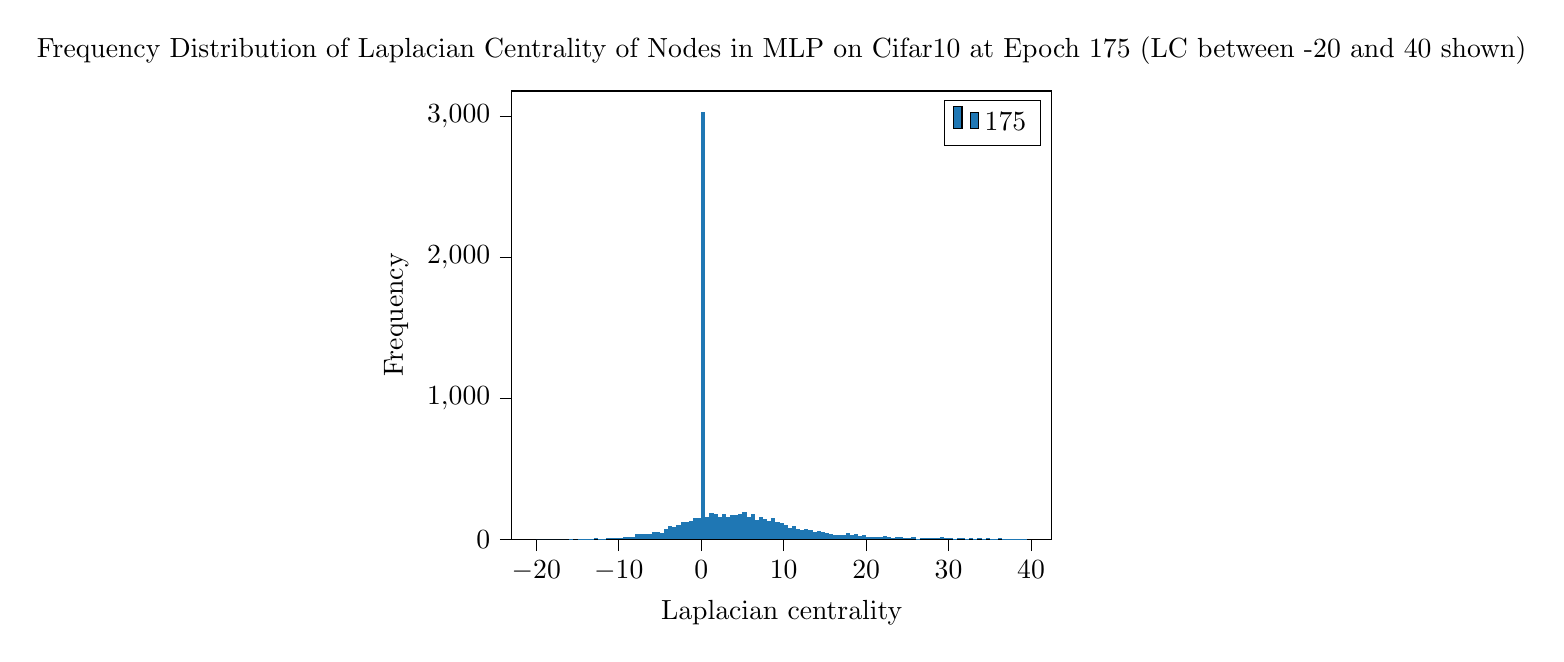
\begin{tikzpicture}

\definecolor{color0}{rgb}{0.12156862745098,0.466666666666667,0.705882352941177}

\begin{axis}[
tick align=outside,
tick pos=left,
title={Frequency Distribution of Laplacian Centrality of Nodes in MLP on Cifar10 at Epoch 175 (LC between -20 and 40 shown)},
x grid style={white!69.0196078431373!black},
xlabel={Laplacian centrality},
xmin=-22.975, xmax=42.475,
xtick style={color=black},
y grid style={white!69.0196078431373!black},
ylabel={Frequency},
ymin=0, ymax=3182.55,
ytick style={color=black}
]
\draw[draw=none,fill=color0] (axis cs:-20,0) rectangle (axis cs:-19.5,0);
\addlegendimage{ybar,ybar legend,draw=none,fill=color0};
\addlegendentry{175}

\draw[draw=none,fill=color0] (axis cs:-19.5,0) rectangle (axis cs:-19,0);
\draw[draw=none,fill=color0] (axis cs:-19,0) rectangle (axis cs:-18.5,0);
\draw[draw=none,fill=color0] (axis cs:-18.5,0) rectangle (axis cs:-18,0);
\draw[draw=none,fill=color0] (axis cs:-18,0) rectangle (axis cs:-17.5,0);
\draw[draw=none,fill=color0] (axis cs:-17.5,0) rectangle (axis cs:-17,0);
\draw[draw=none,fill=color0] (axis cs:-17,0) rectangle (axis cs:-16.5,0);
\draw[draw=none,fill=color0] (axis cs:-16.5,0) rectangle (axis cs:-16,0);
\draw[draw=none,fill=color0] (axis cs:-16,0) rectangle (axis cs:-15.5,1);
\draw[draw=none,fill=color0] (axis cs:-15.5,0) rectangle (axis cs:-15,0);
\draw[draw=none,fill=color0] (axis cs:-15,0) rectangle (axis cs:-14.5,2);
\draw[draw=none,fill=color0] (axis cs:-14.5,0) rectangle (axis cs:-14,1);
\draw[draw=none,fill=color0] (axis cs:-14,0) rectangle (axis cs:-13.5,4);
\draw[draw=none,fill=color0] (axis cs:-13.5,0) rectangle (axis cs:-13,3);
\draw[draw=none,fill=color0] (axis cs:-13,0) rectangle (axis cs:-12.5,7);
\draw[draw=none,fill=color0] (axis cs:-12.5,0) rectangle (axis cs:-12,3);
\draw[draw=none,fill=color0] (axis cs:-12,0) rectangle (axis cs:-11.5,4);
\draw[draw=none,fill=color0] (axis cs:-11.5,0) rectangle (axis cs:-11,9);
\draw[draw=none,fill=color0] (axis cs:-11,0) rectangle (axis cs:-10.5,10);
\draw[draw=none,fill=color0] (axis cs:-10.5,0) rectangle (axis cs:-10,9);
\draw[draw=none,fill=color0] (axis cs:-10,0) rectangle (axis cs:-9.5,11);
\draw[draw=none,fill=color0] (axis cs:-9.5,0) rectangle (axis cs:-9,15);
\draw[draw=none,fill=color0] (axis cs:-9,0) rectangle (axis cs:-8.5,17);
\draw[draw=none,fill=color0] (axis cs:-8.5,0) rectangle (axis cs:-8,15);
\draw[draw=none,fill=color0] (axis cs:-8,0) rectangle (axis cs:-7.5,40);
\draw[draw=none,fill=color0] (axis cs:-7.5,0) rectangle (axis cs:-7,35);
\draw[draw=none,fill=color0] (axis cs:-7,0) rectangle (axis cs:-6.5,37);
\draw[draw=none,fill=color0] (axis cs:-6.5,0) rectangle (axis cs:-6,36);
\draw[draw=none,fill=color0] (axis cs:-6,0) rectangle (axis cs:-5.5,54);
\draw[draw=none,fill=color0] (axis cs:-5.5,0) rectangle (axis cs:-5,55);
\draw[draw=none,fill=color0] (axis cs:-5,0) rectangle (axis cs:-4.5,48);
\draw[draw=none,fill=color0] (axis cs:-4.5,0) rectangle (axis cs:-4,74);
\draw[draw=none,fill=color0] (axis cs:-4,0) rectangle (axis cs:-3.5,96);
\draw[draw=none,fill=color0] (axis cs:-3.5,0) rectangle (axis cs:-3,84);
\draw[draw=none,fill=color0] (axis cs:-3,0) rectangle (axis cs:-2.5,101);
\draw[draw=none,fill=color0] (axis cs:-2.5,0) rectangle (axis cs:-2,120);
\draw[draw=none,fill=color0] (axis cs:-2,0) rectangle (axis cs:-1.5,123);
\draw[draw=none,fill=color0] (axis cs:-1.5,0) rectangle (axis cs:-1,130);
\draw[draw=none,fill=color0] (axis cs:-1,0) rectangle (axis cs:-0.5,149);
\draw[draw=none,fill=color0] (axis cs:-0.5,0) rectangle (axis cs:0,148);
\draw[draw=none,fill=color0] (axis cs:0,0) rectangle (axis cs:0.5,3031);
\draw[draw=none,fill=color0] (axis cs:0.5,0) rectangle (axis cs:1,161);
\draw[draw=none,fill=color0] (axis cs:1,0) rectangle (axis cs:1.5,183);
\draw[draw=none,fill=color0] (axis cs:1.5,0) rectangle (axis cs:2,177);
\draw[draw=none,fill=color0] (axis cs:2,0) rectangle (axis cs:2.5,155);
\draw[draw=none,fill=color0] (axis cs:2.5,0) rectangle (axis cs:3,182);
\draw[draw=none,fill=color0] (axis cs:3,0) rectangle (axis cs:3.5,159);
\draw[draw=none,fill=color0] (axis cs:3.5,0) rectangle (axis cs:4,170);
\draw[draw=none,fill=color0] (axis cs:4,0) rectangle (axis cs:4.5,172);
\draw[draw=none,fill=color0] (axis cs:4.5,0) rectangle (axis cs:5,180);
\draw[draw=none,fill=color0] (axis cs:5,0) rectangle (axis cs:5.5,197);
\draw[draw=none,fill=color0] (axis cs:5.5,0) rectangle (axis cs:6,161);
\draw[draw=none,fill=color0] (axis cs:6,0) rectangle (axis cs:6.5,179);
\draw[draw=none,fill=color0] (axis cs:6.5,0) rectangle (axis cs:7,134);
\draw[draw=none,fill=color0] (axis cs:7,0) rectangle (axis cs:7.5,159);
\draw[draw=none,fill=color0] (axis cs:7.5,0) rectangle (axis cs:8,146);
\draw[draw=none,fill=color0] (axis cs:8,0) rectangle (axis cs:8.5,133);
\draw[draw=none,fill=color0] (axis cs:8.5,0) rectangle (axis cs:9,151);
\draw[draw=none,fill=color0] (axis cs:9,0) rectangle (axis cs:9.5,122);
\draw[draw=none,fill=color0] (axis cs:9.5,0) rectangle (axis cs:10,112);
\draw[draw=none,fill=color0] (axis cs:10,0) rectangle (axis cs:10.5,103);
\draw[draw=none,fill=color0] (axis cs:10.5,0) rectangle (axis cs:11,81);
\draw[draw=none,fill=color0] (axis cs:11,0) rectangle (axis cs:11.5,94);
\draw[draw=none,fill=color0] (axis cs:11.5,0) rectangle (axis cs:12,73);
\draw[draw=none,fill=color0] (axis cs:12,0) rectangle (axis cs:12.5,66);
\draw[draw=none,fill=color0] (axis cs:12.5,0) rectangle (axis cs:13,72);
\draw[draw=none,fill=color0] (axis cs:13,0) rectangle (axis cs:13.5,64);
\draw[draw=none,fill=color0] (axis cs:13.5,0) rectangle (axis cs:14,51);
\draw[draw=none,fill=color0] (axis cs:14,0) rectangle (axis cs:14.5,57);
\draw[draw=none,fill=color0] (axis cs:14.5,0) rectangle (axis cs:15,52);
\draw[draw=none,fill=color0] (axis cs:15,0) rectangle (axis cs:15.5,42);
\draw[draw=none,fill=color0] (axis cs:15.5,0) rectangle (axis cs:16,37);
\draw[draw=none,fill=color0] (axis cs:16,0) rectangle (axis cs:16.5,33);
\draw[draw=none,fill=color0] (axis cs:16.5,0) rectangle (axis cs:17,32);
\draw[draw=none,fill=color0] (axis cs:17,0) rectangle (axis cs:17.5,32);
\draw[draw=none,fill=color0] (axis cs:17.5,0) rectangle (axis cs:18,44);
\draw[draw=none,fill=color0] (axis cs:18,0) rectangle (axis cs:18.5,31);
\draw[draw=none,fill=color0] (axis cs:18.5,0) rectangle (axis cs:19,38);
\draw[draw=none,fill=color0] (axis cs:19,0) rectangle (axis cs:19.5,24);
\draw[draw=none,fill=color0] (axis cs:19.5,0) rectangle (axis cs:20,27);
\draw[draw=none,fill=color0] (axis cs:20,0) rectangle (axis cs:20.5,18);
\draw[draw=none,fill=color0] (axis cs:20.5,0) rectangle (axis cs:21,18);
\draw[draw=none,fill=color0] (axis cs:21,0) rectangle (axis cs:21.5,16);
\draw[draw=none,fill=color0] (axis cs:21.5,0) rectangle (axis cs:22,14);
\draw[draw=none,fill=color0] (axis cs:22,0) rectangle (axis cs:22.5,20);
\draw[draw=none,fill=color0] (axis cs:22.5,0) rectangle (axis cs:23,15);
\draw[draw=none,fill=color0] (axis cs:23,0) rectangle (axis cs:23.5,7);
\draw[draw=none,fill=color0] (axis cs:23.5,0) rectangle (axis cs:24,19);
\draw[draw=none,fill=color0] (axis cs:24,0) rectangle (axis cs:24.5,13);
\draw[draw=none,fill=color0] (axis cs:24.5,0) rectangle (axis cs:25,10);
\draw[draw=none,fill=color0] (axis cs:25,0) rectangle (axis cs:25.5,10);
\draw[draw=none,fill=color0] (axis cs:25.5,0) rectangle (axis cs:26,13);
\draw[draw=none,fill=color0] (axis cs:26,0) rectangle (axis cs:26.5,3);
\draw[draw=none,fill=color0] (axis cs:26.5,0) rectangle (axis cs:27,11);
\draw[draw=none,fill=color0] (axis cs:27,0) rectangle (axis cs:27.5,9);
\draw[draw=none,fill=color0] (axis cs:27.5,0) rectangle (axis cs:28,9);
\draw[draw=none,fill=color0] (axis cs:28,0) rectangle (axis cs:28.5,7);
\draw[draw=none,fill=color0] (axis cs:28.5,0) rectangle (axis cs:29,8);
\draw[draw=none,fill=color0] (axis cs:29,0) rectangle (axis cs:29.5,13);
\draw[draw=none,fill=color0] (axis cs:29.5,0) rectangle (axis cs:30,8);
\draw[draw=none,fill=color0] (axis cs:30,0) rectangle (axis cs:30.5,12);
\draw[draw=none,fill=color0] (axis cs:30.5,0) rectangle (axis cs:31,5);
\draw[draw=none,fill=color0] (axis cs:31,0) rectangle (axis cs:31.5,8);
\draw[draw=none,fill=color0] (axis cs:31.5,0) rectangle (axis cs:32,11);
\draw[draw=none,fill=color0] (axis cs:32,0) rectangle (axis cs:32.5,5);
\draw[draw=none,fill=color0] (axis cs:32.5,0) rectangle (axis cs:33,6);
\draw[draw=none,fill=color0] (axis cs:33,0) rectangle (axis cs:33.5,5);
\draw[draw=none,fill=color0] (axis cs:33.5,0) rectangle (axis cs:34,6);
\draw[draw=none,fill=color0] (axis cs:34,0) rectangle (axis cs:34.5,5);
\draw[draw=none,fill=color0] (axis cs:34.5,0) rectangle (axis cs:35,7);
\draw[draw=none,fill=color0] (axis cs:35,0) rectangle (axis cs:35.5,1);
\draw[draw=none,fill=color0] (axis cs:35.5,0) rectangle (axis cs:36,3);
\draw[draw=none,fill=color0] (axis cs:36,0) rectangle (axis cs:36.5,6);
\draw[draw=none,fill=color0] (axis cs:36.5,0) rectangle (axis cs:37,4);
\draw[draw=none,fill=color0] (axis cs:37,0) rectangle (axis cs:37.5,2);
\draw[draw=none,fill=color0] (axis cs:37.5,0) rectangle (axis cs:38,4);
\draw[draw=none,fill=color0] (axis cs:38,0) rectangle (axis cs:38.5,5);
\draw[draw=none,fill=color0] (axis cs:38.5,0) rectangle (axis cs:39,2);
\draw[draw=none,fill=color0] (axis cs:39,0) rectangle (axis cs:39.5,3);
\end{axis}

\end{tikzpicture}
